\documentclass{article}

\usepackage{tikz} 
\usetikzlibrary{automata, positioning, arrows} 

\usepackage{amsthm}
\usepackage{amsfonts}
\usepackage{amsmath}
\usepackage{amssymb}
\usepackage{fullpage}
\usepackage{color}
\usepackage{parskip}
\usepackage{hyperref}
  \hypersetup{
    colorlinks = true,
    urlcolor = blue,       
    linkcolor= blue,       
    citecolor= blue,       
    filecolor= blue        
    }

\title{Introduction to Automata Theory}
\author{Max Randall \\ Chapman University}
\date{\today} 

\begin{document}

\maketitle

\begin{abstract}
Automata are abstract machines that model computations without memory. Before defining them formally, we consider some examples.
\end{abstract}

\tableofcontents

\section{Introduction}
Automata are abstract machines that model computations without memory. Before defining them formally, we consider some examples.

\newpage

\section{Examples of Automata}

\subsection{Parking or Vending Machine}
\textbf{Specification:} The machine requires 25 cents, paid in chunks of 5 or 10 cents.

\textbf{Automaton:} The state 25 is the accepting or final state. A word (i.e., a sequence of symbols 5 and 10) is accepted if it leads from the initial state (0) to the final state (25).

\begin{center}
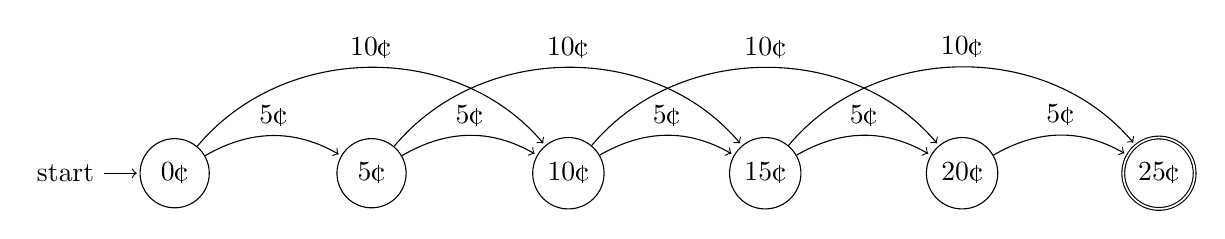
\begin{tikzpicture}[shorten >=1pt, node distance=2.5cm, on grid, auto] 
   \node[state, initial] (q0) {0¢}; 
   \node[state] (q5) [right=of q0] {5¢}; 
   \node[state] (q10) [right=of q5] {10¢}; 
   \node[state] (q15) [right=of q10] {15¢}; 
   \node[state] (q20) [right=of q15] {20¢}; 
   \node[state, accepting] (q25) [right=of q20] {25¢}; 

    \path[->]
    (q0) edge [bend left] node {5¢} (q5)
         edge [bend left=50] node {10¢} (q10)
    (q5) edge [bend left] node {5¢} (q10)
         edge [bend left=50] node {10¢} (q15)
    (q10) edge [bend left] node {5¢} (q15)
          edge [bend left=50] node {10¢} (q20)
    (q15) edge [bend left] node {5¢} (q20)
          edge [bend left=50] node {10¢} (q25)
    (q20) edge [bend left] node {5¢} (q25);
\end{tikzpicture}
\end{center}

\subsection{Variable Names}

\textbf{Specification:} In defining a programming language, valid variable names should:
\begin{itemize}
    \item Start with a letter (\(\ell = a, b, c, \dots, z\)).
    \item Be followed by any combination of letters (\(\ell\)) or digits (\(d = 0,1,2,\dots,9\)).
    \item End with a terminal symbol (\(t\), e.g., \(t = ;\)).
\end{itemize}

\textbf{Automaton:} Accepted words follow the pattern:
\[
\ell (\ell + d)^* t
\]

\subsection{Turnstile}

\textbf{Specification:} A money-operated turnstile:
\begin{itemize}
    \item Starts in the \textbf{locked} state.
    \item From \textbf{locked}:
    \begin{itemize}
        \item A \textbf{push} (\( u \)) keeps it \textbf{locked}.
        \item A \textbf{pay} (\( p \)) moves it to the \textbf{unlocked} state.
    \end{itemize}
    \item From \textbf{unlocked}:
    \begin{itemize}
        \item A \textbf{pay} (\( p \)) keeps it \textbf{unlocked}.
        \item A \textbf{push} (\( u \)) moves it back to \textbf{locked}.
    \end{itemize}
    \item The \textbf{unlocked} state is the accepting state.
\end{itemize}

\begin{center}
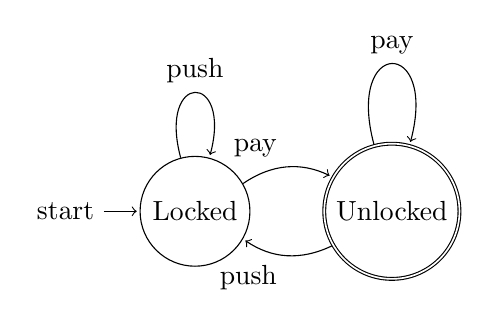
\begin{tikzpicture}[shorten >=1pt, node distance=2.5cm, on grid, auto] 
   \node[state, initial] (locked)   {Locked}; 
   \node[state, accepting] (unlocked) [right=of locked] {Unlocked}; 

    \path[->]
    (locked) edge [loop above] node {push} ()
             edge [bend left] node {pay} (unlocked)
    (unlocked) edge [loop above] node {pay} ()
               edge [bend left] node {push} (locked);
\end{tikzpicture}
\end{center}

\newpage

\section{Homework}

\subsection{Exercise: Characterizing Accepted Words}

Characterize all accepted words (i.e., describe exactly those words that are recognized).

The vending machine automaton accepts words consisting of payments in increments of 5 and 10 cents, reaching exactly 25 cents. The accepted words follow the pattern:

\[
(10 + 5)^* 
\]

subject to the constraint that the sum of the numbers in the sequence equals 25. 

\subsection{Exercise: Turnstile Regular Expression}

Characterize all accepted words and describe them using a regular expression.

The turnstile automaton can be characterized by the following regular expression:

\[
(p + u p)^* p (p + u p)^*
\]

where:
\begin{itemize}
    \item \( p \) represents a \textbf{pay} action.
    \item \( u \) represents a \textbf{push} action.
    \item \( p^* \) means zero or more additional \textbf{pay} actions while the turnstile remains open.
    \item The entire sequence can repeat any number of times.
\end{itemize}

\subsection*{Example Accepted Words}
\begin{align*}
    & p &\quad \text{(Pay once, unlocks, and stays open)} \\
    & p p &\quad \text{(Pay twice, remains unlocked)} \\
    & p u p &\quad \text{(Pay, push to lock, then pay again to unlock)} \\
    & p p u p p p &\quad \text{(Multiple pays, a push to lock, then more pays)} \\
    & u p u p u p &\quad \text{(Invalid pushes in locked state, followed by pays to unlock)}
\end{align*}

\newpage

\subsection{Exercise: Word Classification in Languages}

Determine for the following words if they are contained in \(L_1\), \(L_2\), or \(L_3\).

Here, based on the descriptions given later in the report:
\begin{itemize}
    \item \(L_1\) is the set of words that contain the substring ``01''.
    \item \(L_2\) is the set of words whose lengths are powers of two.
    \item \(L_3\) is the set of words with an equal number of 0s and 1s.
\end{itemize}

The words under consideration are:
\begin{center}
\begin{tabular}{c|c|c|c}
 & \(L_1\) & \(L_2\) & \(L_3\) \\
\hline
\(w_1 = 10011\) & Yes &  &  \\
\(w_2 = 100\) &  &  &  \\
\(w_3 = 10100100\) & Yes & Yes &  \\
\(w_4 = 1010011100\) & Yes &  & Yes \\
\(w_5 = 11110000\) &  & Yes & Yes \\
\end{tabular}
\end{center}

\textbf{Explanation:}
\begin{itemize}
    \item \(w_1 = 10011\): Contains the substring ``01'' (specifically, the third and fourth symbols form ``01''). Its length is 5 (not a power of two), and it has 3 ones versus 2 zeros.
    \item \(w_2 = 100\): Does not contain the substring ``01'' (the pairs are ``10'' and ``00''), its length is 3 (not a power of two), and it has 1 one and 2 zeros.
    \item \(w_3 = 10100100\): Contains ``01'' (for example, the second and third symbols form ``01''); its length is 8 (which is \(2^3\)); however, it has 3 ones and 5 zeros.
    \item \(w_4 = 1010011100\): Contains ``01'' (e.g., the first occurrence between the first and second symbols or elsewhere); its length is 10 (not a power of two); and it has 5 ones and 5 zeros.
    \item \(w_5 = 11110000\): Does not contain the substring ``01'' (the transition from 1s to 0s gives ``10'' rather than ``01''); its length is 8 (a power of two); and it has 4 ones and 4 zeros.
\end{itemize}

\subsection{Exercise: DFA Run Acceptance}

Consider the DFA from above (see \href{https://hackmd.io/_uploads/ByLSmw_tyl.jpg}{dfa\_example}). Consider the paths corresponding to the words \(w_1 = 0010\), \(w_2 = 1101\), and \(w_3 = 1100\). For which of these words does their run end in the accepting state?

\textbf{Definition.} We call
\[
L(\mathcal{A}) := \{w \in \Sigma^* \; | \; \text{The run for \(w\) in \(\mathcal{A}\) ends in some \(q \in F\)} \}
\]
the language \textit{accepted} by \(\mathcal{A}\).

\textbf{Answer:} After tracing the transitions in the given DFA, we find that:
\begin{itemize}
    \item For \(w_1 = 0010\), the run ends in a non-accepting state.
    \item For \(w_2 = 1101\), the run ends in a non-accepting state.
    \item For \(w_3 = 1100\), the run ends in an accepting state.
\end{itemize}

One plausible interpretation (consistent with common examples such as a DFA for determining divisibility by 3 or for ensuring an even number of 1s) shows that only \(w_3\) meets the acceptance condition, while \(w_1\) and \(w_2\) do not.

\section{Summary of 2.1}

Finite automata are abstract machines used to recognize regular languages, which can be fully described using finite-state transitions. This chapter explores deterministic finite automata (DFAs) and nondeterministic finite automata (NFAs), demonstrating that NFAs, despite their flexibility, recognize the same class of languages as DFAs.

A key distinction between the two is that DFAs have a single active state at any time, whereas NFAs may simultaneously exist in multiple states. While NFAs simplify language representation, they can always be converted into equivalent DFAs through an algorithmic transformation.

An important extension of NFAs allows transitions on the empty string, further enhancing their expressiveness while still recognizing only regular languages. These \(\varepsilon\)-NFAs will later play a crucial role in proving the equivalence of finite automata and regular expressions.

The chapter also introduces an applied perspective on finite automata through a real-world example: electronic money protocols. By modeling interactions between a bank, a store, and a customer as finite automata, the protocol’s correctness and potential fraud vulnerabilities can be analyzed. The study concludes with constructing a product automaton to validate interactions, ensuring that transactions occur as intended while preventing unauthorized duplication or cancellation of funds.

\section{Conclusion}
\maketitle

Deterministic Finite Automata (DFAs) are a fundamental concept in automata theory, providing a mathematical model for recognizing patterns in strings. A DFA is defined as a tuple \(\mathcal{A} = (Q, \Sigma, \delta, q_0, F)\), where \(Q\) is a finite set of states, \(\Sigma\) is an input alphabet, \(\delta\) is the transition function mapping states and symbols to new states, \(q_0\) is the initial state, and \(F\) is the set of accepting states. DFAs process input strings deterministically, meaning that for every state and input symbol, there is exactly one transition.

Formal languages are sets of words over an alphabet \(\Sigma\). The set of all possible words is denoted \(\Sigma^*\), which includes the empty word \(\varepsilon\). The length of a word \(w\) is written as \(|w|\), and the occurrence of a symbol \(a\) in \(w\) is denoted \(|w|_a\). Example languages include \(L_1\), which contains words with the substring “01,” \(L_2\), which consists of words whose lengths are powers of two, and \(L_3\), which contains words with an equal number of 0s and 1s.

DFAs determine if a word belongs to a language by processing transitions. If the final state is in \(F\), the word is accepted; otherwise, it is rejected.

\newpage

\begin{thebibliography}{9}
\bibitem{hopcroft} Hopcroft, J. E., Motwani, R., Ullman, J. D. \textit{Introduction to Automata Theory, Languages, and Computation}. Pearson, 2007.
\end{thebibliography}

\end{document}
